
\chapter{束流模拟程序的物理模型和算法}
\label{chap:Algorithm}
空间电荷效应是束流物理中非常重要的问题。特别是对于强流加速器,空间电荷效应更加明显,因此我们必须在加速器设计中正确处理。
如我们在\eqref{section:spaceChargeIntro}节中所介绍,目前存在若干种不同的计算空间电荷效应的模型,
比如线性近似、P2P方法、PIC模型、Symplectic模型,各个模型的计算速度、精度、近似程度都有所不同。

在本章中,主要介绍计算空间电荷效应的几种物理模型和模拟程序的一般性设计准则。
首先,节\eqref{section:particle_core}对一种近似求解单粒子空间电荷效应的物理模型 - 束核模型 - 进行介绍。
其次,在\eqref{section:PIC_algorithm}节中对束流模拟中的经典的PIC算法进行介绍。
之后,在\eqref{section:symplectic_theory}节中对一种新型的求解空间电荷效应的算法 - Symplectic算法 - 进行介绍。
%最后,我们在\eqref{section:GPU_CPU}节中对不同的计算机并行结构进行一些比较。
最后,\eqref{section:Algorithm_conclusion}节中对各个物理模型进行了小结。

\section{束核模型}            \label{section:particle_core}
%针对空间电荷问题,我们主要有两种描述手段:解析的方法和数值的方法。其中解析的方法为求解弗拉索夫方程(弗拉索夫 Equation),如式\eqref{eq:弗拉索夫}:
%\begin{equation}
%    \label{eq:弗拉索夫}
%    \begin{aligned}
%        & f(x,y,z,{{p}_{x}},{{p}_{y}},{{p}_{z}})=f(H) \\
%        & \frac{df}{dt}=0 \\
%        & \Delta U=-\frac{\rho }{{{\varepsilon }_{0}}} \\
%    \end{aligned}
%\end{equation}
由于空间电荷效应这个多体耦合问题没有解析解,所以我们必须采用一些近似,建立一个更简单的模型,以得到这个问题的大致图像。
R. L. Gluckstern和T. P. Wangler等人提出了一种束核模型(particle-core)\cite{gluckstern1994analytic,wangler1998particle},以描述空间电荷导致的束晕形成机制\cite{chen1995self,okamoto1997simulation,gluckstern1998halo,fedotov1999halo,qiang2000beam}。
在束核模型中连续的束流通过一个轴对称的聚焦通道,假设粒子束核为均匀分布,则其包络大小可由包络方程描述。此时一个任意的粒子会受到束核产生的空间电荷力,当粒子处于束核内部时,空间电荷力为线性的;当粒子处于束核外部时,空间电荷力为非线性的。
忽略单粒子对束核的影响,则束核的半径可以由下式表示:
\begin{equation}
    \label{eq:particle_core_envelope}
    \frac{{{d}^{2}}R}{d{{z}^{2}}}+k_{0}^{2}R-\frac{{{\varepsilon }^{2}}}{{{R}^{3}}}-\frac{K}{R}=0,
\end{equation}
其中
\begin{equation}
K=\frac{qI}{2\pi \varepsilon {m_0}{{c}^{3}}{{\beta }^{3}}{{\gamma }^{3}}}\text{。}
\end{equation}
其中$R$为束核包络的大小,$q$,$m_0$,和$\beta c$分别为粒子的电荷,质量,和运动速度,$k_{0}$为外部聚焦强度,$\gamma$为洛伦兹因子,$I$为流强,$\varepsilon$为发射度。

所以,单粒子的横向运动方程可以表示为:
\begin{equation}
    \label{eq:particle_core_singleparticle}
    \frac{{{\text{d}}^{2}}X}{\text{d}{{z}^{2}}}+k_{0}^{2}X-{{F}_{sc}}=0,
\end{equation}
其中,$X$为粒子的横向位置,${F}_{sc}$为由均匀分布束核产生的空间电荷力,可以表示为:
\begin{equation}
{{F}_{sc}}=\left\{
        \begin{aligned}
        & KX/{{R}^{2}}, &\left| X \right|<R \\
        & K/X,          &\left| X \right|\ge R \\
        \end{aligned} \right. \text{。}
\end{equation}

对式\eqref{eq:particle_core_envelope}和式\eqref{eq:particle_core_singleparticle}进行无量纲化,我们引入变量~$r=R/R_0$,$x=X/R_0$,$\tau = k_0 z $,
并将空间电荷导致的tune depression表示为~$\eta = k/k_0 = \sqrt{1+u^2}-u$。则无量纲化的束核包络方程可以表示为:
\begin{equation}
    \label{eq:particle_core_envelope_dimensionless}
    \frac{{{d}^{2}}r}{d{{\tau}^{2}}}+r-\frac{{{\eta }^{2}}}{{{r}^{3}}}-\frac{1-{\eta}^2}{r}=0 \text{。}
\end{equation}
无量纲化的单粒子运动方程可以表示为:
\begin{equation}
    \label{eq:particle_core_singleparticle_dimensionless}
    \frac{{{d}^{2}}x}{d{{\tau}^{2}}}+x = (1-{\eta}^2) \times \left\{
        \begin{aligned}
        & x/{{r}^{2}}, &\left| x \right|<r \\
        & 1/x,         &\left| x \right|\ge r \\
        \end{aligned} \right. \text{。}
\end{equation}

式\eqref{eq:particle_core_envelope_dimensionless}和
式\eqref{eq:particle_core_singleparticle_dimensionless}仅含有相位压缩因子$\eta$一个参数。
当$r_0=1$时,束流包络为常数,即束核匹配。为了描述束核的初始匹配程度,我们将束核的初始的包络半径定位为失配度$\mu = r_{0}$。
失配度会影响束核包络的变化。当束核完全与聚焦强度相匹配时,即$\mu = 1$时,束核的包络大小是不变的;
而当包络与聚焦强度不匹配的时候,包络半径会发生周期性变化。
图\eqref{fig:particle_core_envelope}为束核包络与单粒子横向位移示意图,其横坐标为周期数,纵坐标为粒子位置或束团半径,单位为米。
其中蓝色曲线为$\eta = 0.5$,$\mu = 0.6$时的束核半径变化情况,红色曲线为初始条件为$x=0.8$,$x'=0$的粒子横向轨迹。
可以看出,束核的半径呈现规律的周期振荡,而粒子和束核的相互作用会驱使粒子横向位置发生变化,以表示空间电荷对粒子的影响。
\begin{figure}[!tbh]
    \centering
    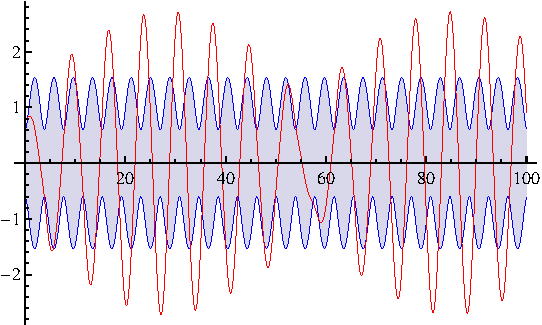
\includegraphics[width=0.65\textwidth]{Img/particle_core_envelope.pdf}
    \caption{束核包络与单粒子横向位移示意图}
    \label{fig:particle_core_envelope}
\end{figure}

图\eqref{fig:particle_core_particle}为每个周期的开始处粒子的相空间位置,
其中横轴为粒子横向位置,纵轴为粒子横向动量,这张图被称为粒子的庞加莱截面(Poincaré surface of section)。
在庞加莱截面中可以看到明显的规律,粒子沿着其中一条轨道进行运动。
\begin{figure}[!tbh]
    \centering
    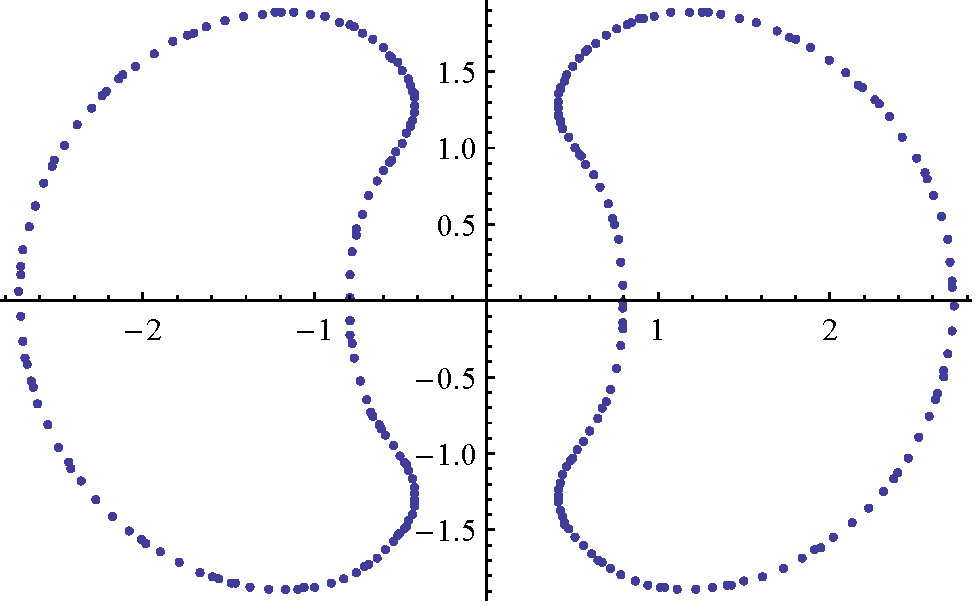
\includegraphics[width=0.65\textwidth]{Img/particle_core_particle.pdf}
    \caption{粒子的庞加莱截面示意图}
    \label{fig:particle_core_particle}
\end{figure}

图\eqref{fig:particle_core_Poincare}中的三幅图分别为不同的相位压缩因子$\eta$下的一组庞加莱截面,
其中每一张图中的不同的颜色的点代表不同的初始相空间位置的粒子的轨迹。
可以看出,庞加莱截面图可以分为三个区域:(1)内椭圆区,其大小约为束核半径及周边一小部分;
(2)不动点区,或者叫共振区,包括x轴上的不动点以及周围的环线,其显示了参数共振的轨迹;(3)外部类椭圆轨迹。
在空间电荷效应较弱的情况下,即$\eta$较大时,三个区的粒子都是作有规律的运动,如图\eqref{fig:particle_core_Poincare5}所示。
但是当空间电荷主导的时候,比如$\eta=0.1$时(图\eqref{fig:particle_core_Poincare1}),
在内椭圆区会出现混沌行为,并且随着相位压缩因子变小,混沌行为变得更加明显,参数区的粒子轨迹也开始对初始条件敏感。
\begin{figure}[!htbp]
  \centering
  ~%add desired spacing
  \begin{subfigure}[b]{0.6\textwidth}
    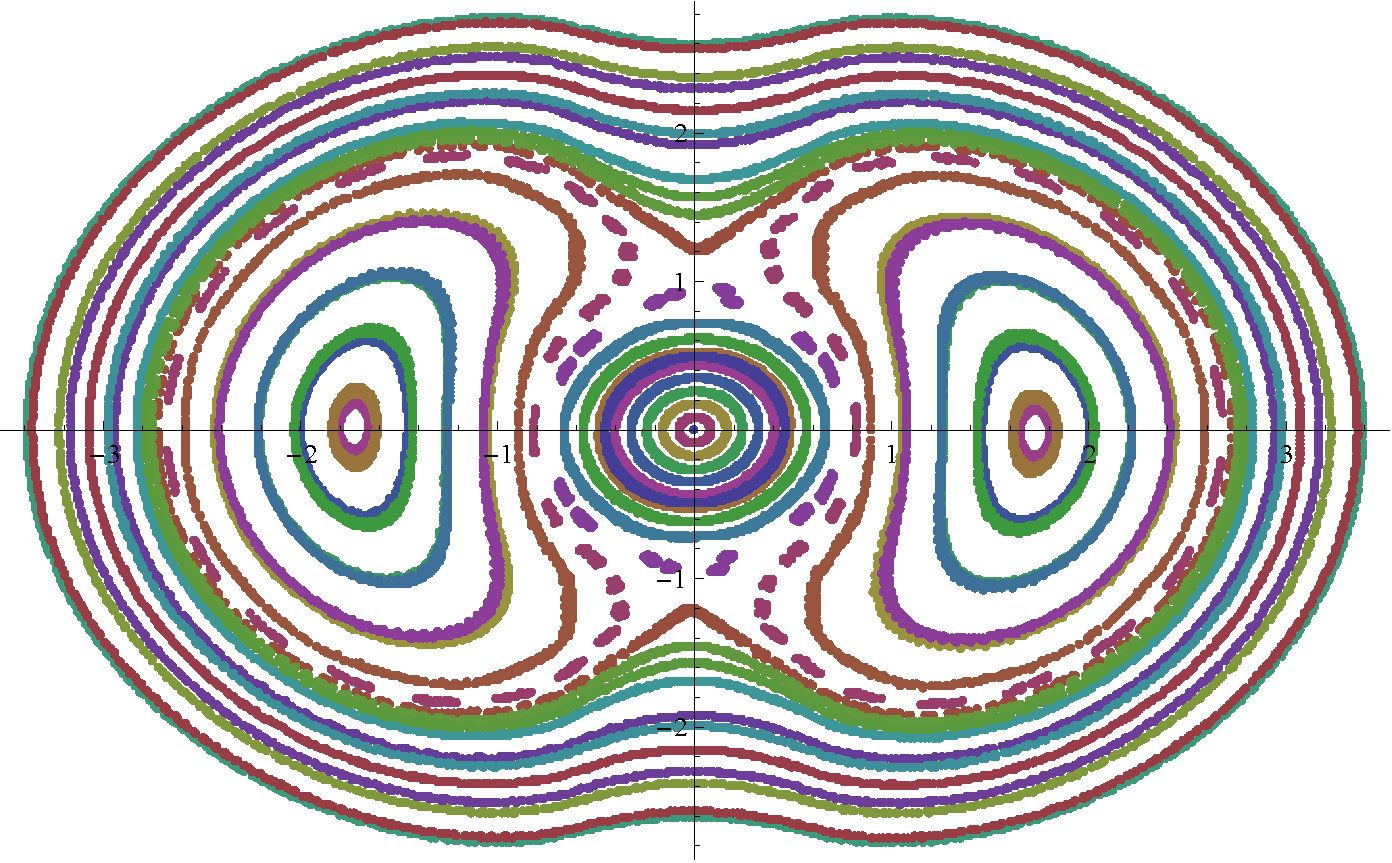
\includegraphics[width=\textwidth]{particle_core_Poincare5.pdf}
    \caption{$\eta = 0.5$}
    \label{fig:particle_core_Poincare5}
  \end{subfigure}
  ~
  \begin{subfigure}[b]{0.6\textwidth}
    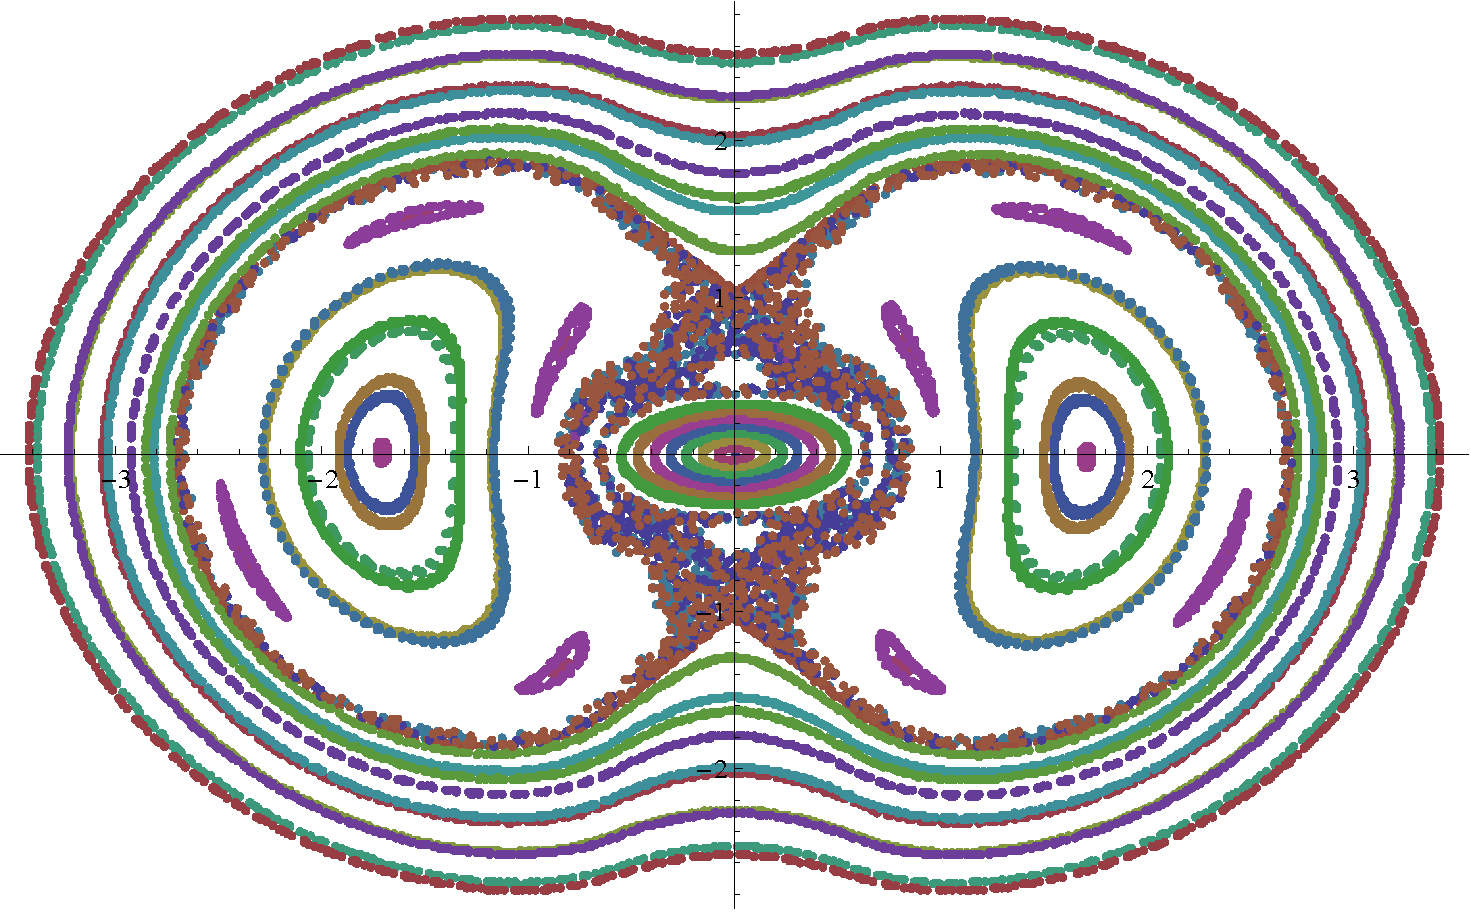
\includegraphics[width=\textwidth]{particle_core_Poincare3.pdf}
    \caption{$\eta = 0.3$}
    \label{fig:particle_core_Poincare3}
  \end{subfigure}%
  ~
  \begin{subfigure}[b]{0.6\textwidth}
    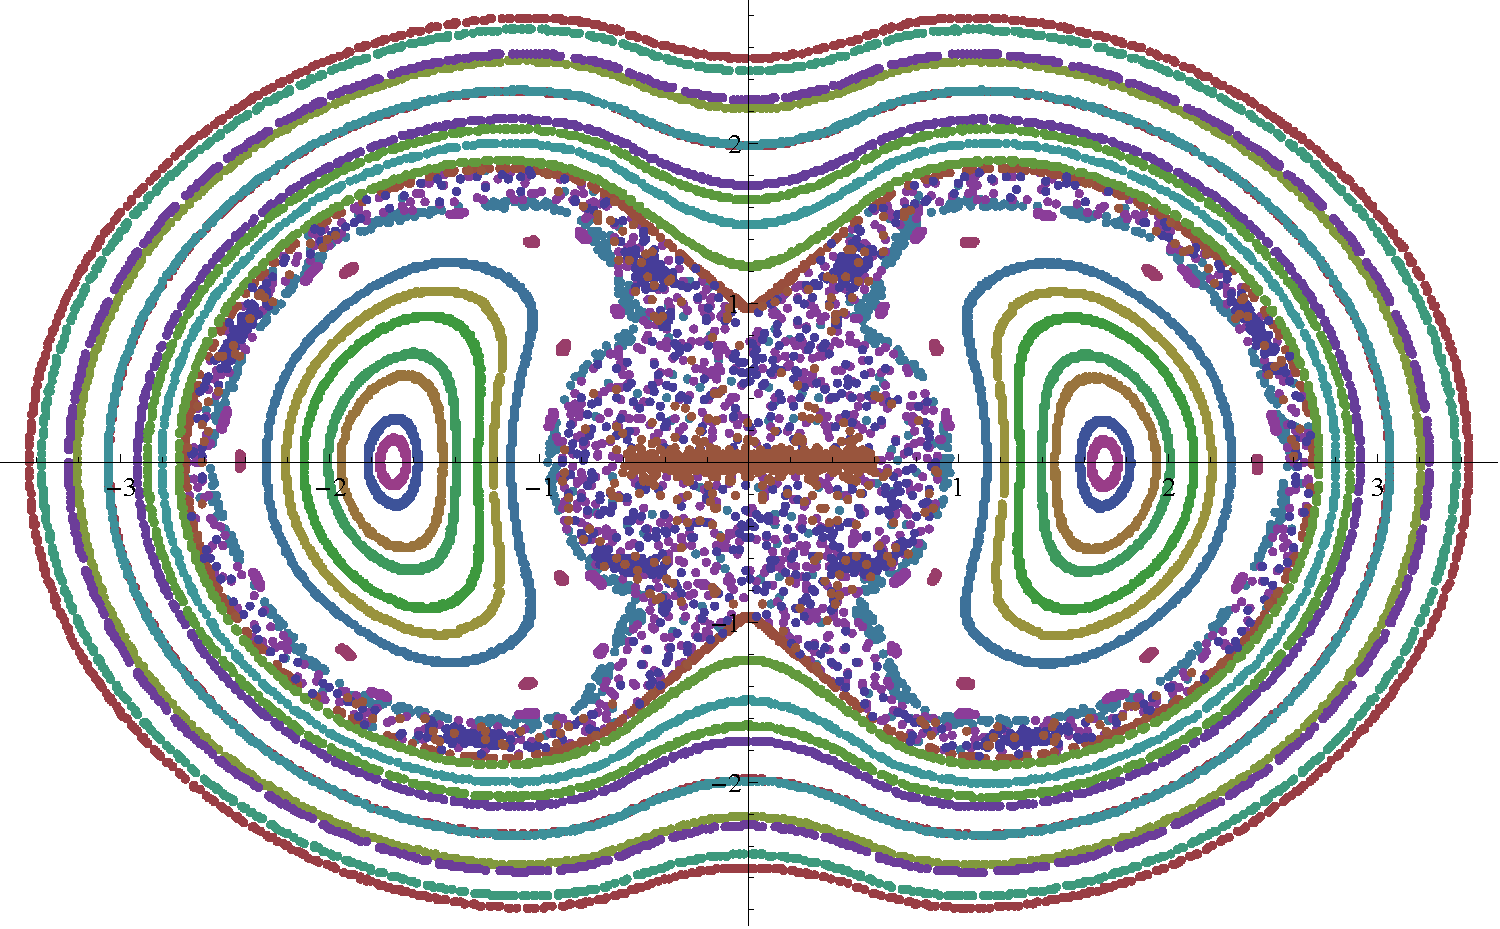
\includegraphics[width=\textwidth]{particle_core_Poincare1.pdf}
    \caption{$\eta = 0.1$}
    \label{fig:particle_core_Poincare1}
  \end{subfigure}%
  \caption{不同相位压缩因子下的庞加莱截面}
  \label{fig:particle_core_Poincare}
\end{figure}
采用庞加莱截面我们可以对束晕形成的机制进行分析。
束晕中的粒子主要来源于共振区中的粒子。
这些粒子最开始分布于内椭圆区与共振区的分界线附近,随着粒子运动,其向外移动到共振区与外椭圆区的边界附近,在两个边界间振荡,形成了束晕。
在空间电荷效应主导的情况下,内椭圆区的粒子也有可能形成束晕。
比如图\eqref{fig:particle_core_Poincare1}中的内椭圆区也出现了混沌行为,因此最内部的粒子也会移动到外部形成束晕。

束核模型在一定程度上可以解释束晕形成的机制,但是这个模型并不是自洽的,与实际不相符。
束核模型假设束核是稳定的,并且外部聚焦力是恒定的常数;
而实际的束核有可能是不稳定的,外部的聚焦力也是可能变化的。
因此,我们需要一个更加自洽的系统来研究束流的行为。

\section{束流模拟原理及PIC算法}    \label{section:PIC_algorithm}
PIC算法是一种使用自洽的系统研究空间电荷效应的一种数值模拟算法\cite{hockney1988computer,PIC_luccio2002space}。
PIC发展于上世纪七十年代,被广泛的应用于等离子体和加速器束流的模拟与研究。
目前,主流的加速器模拟程序都是使用的PIC算法求解空间电荷效应\cite{PIC_Birdsall1991, PIC_friedman1992, PIC_ji2000, PIC_ji2004, PIC_Amundson2006229, PIC_tracewin2014, PIC_beampath2005}。
使用PIC算法进行束流模拟的基本流程如图\eqref{fig:PICflow1}和\eqref{fig:PICflow2}所示。

\begin{figure}[!tbh]
%to be modified
  \centering
    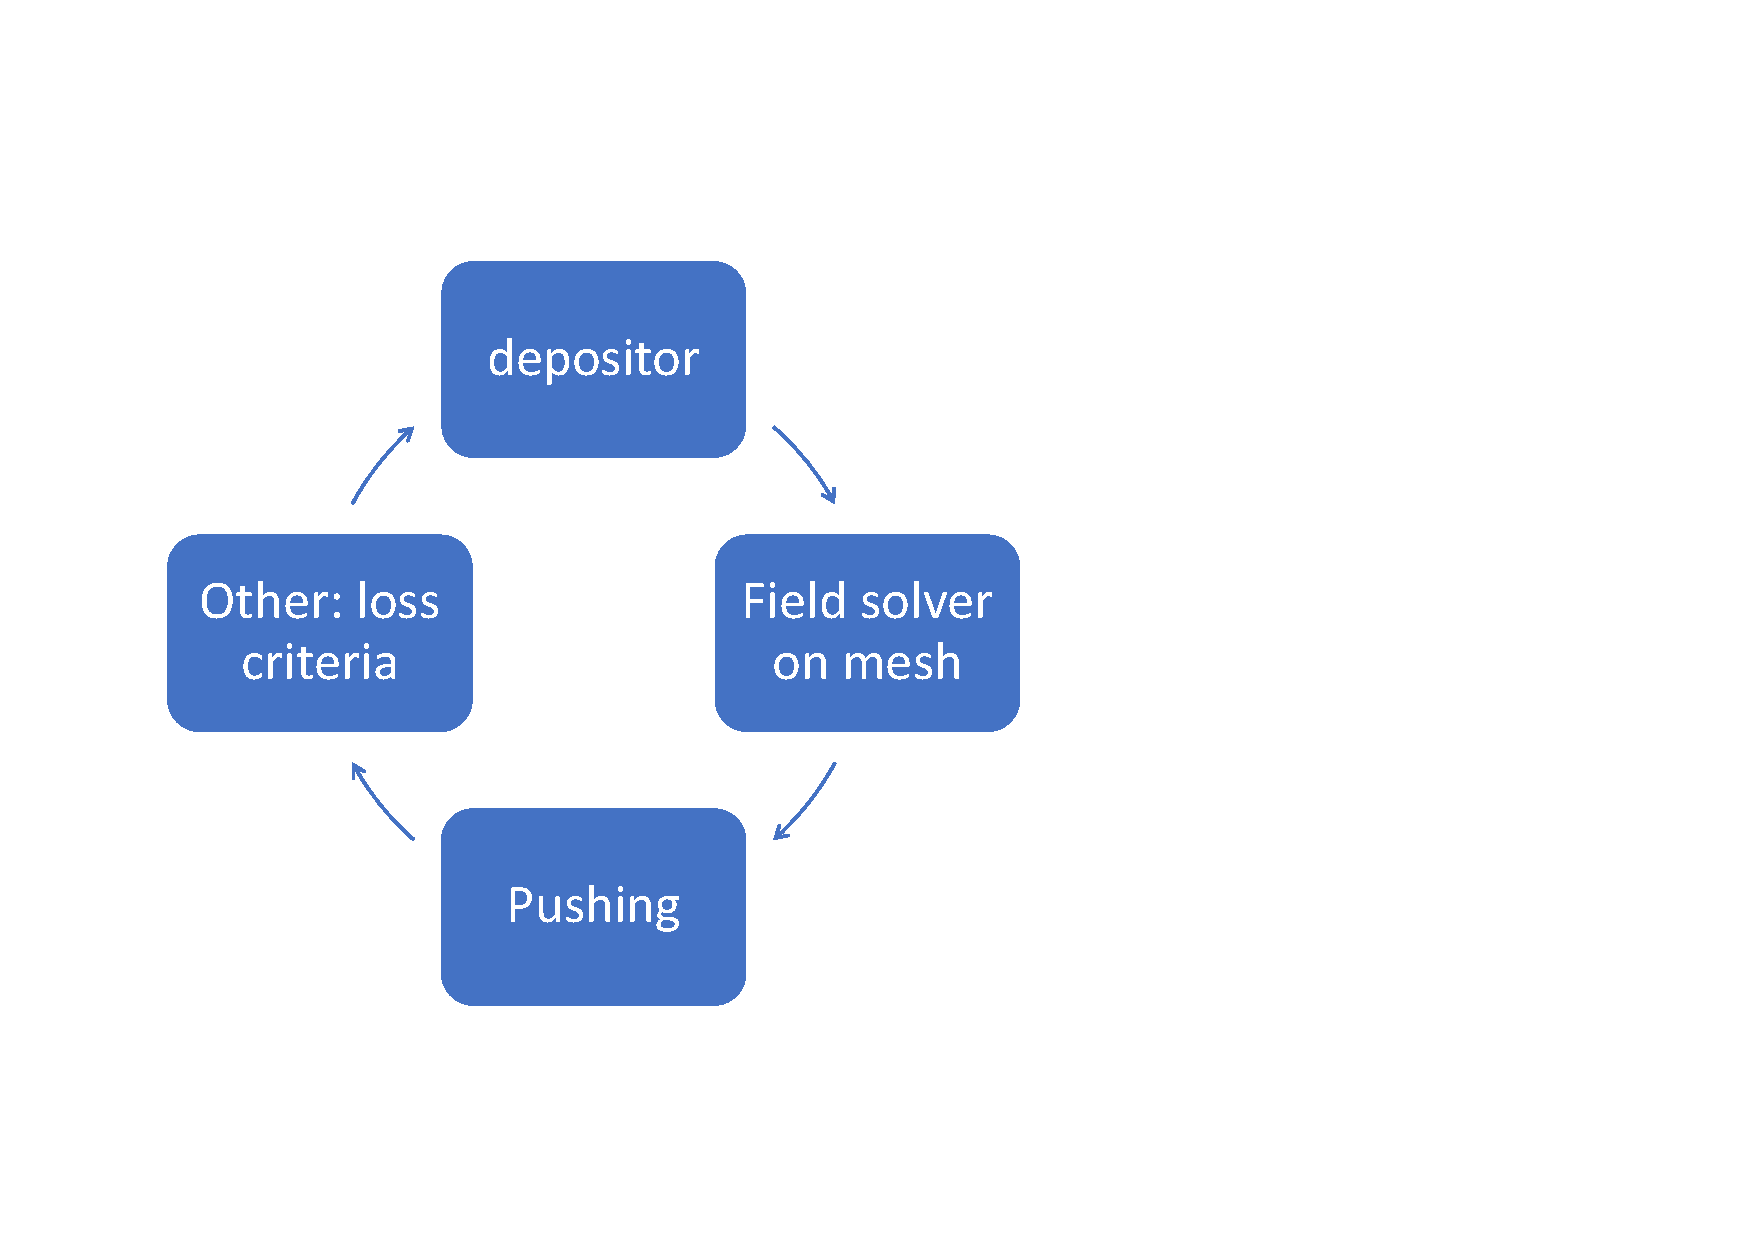
\includegraphics[width=0.5\textwidth]{Img/3_1_PIC.pdf}
    \caption{PIC算法块循环示意图}
    \label{fig:PICflow1}
\end{figure}

\begin{figure}[!tbh]
  \centering
    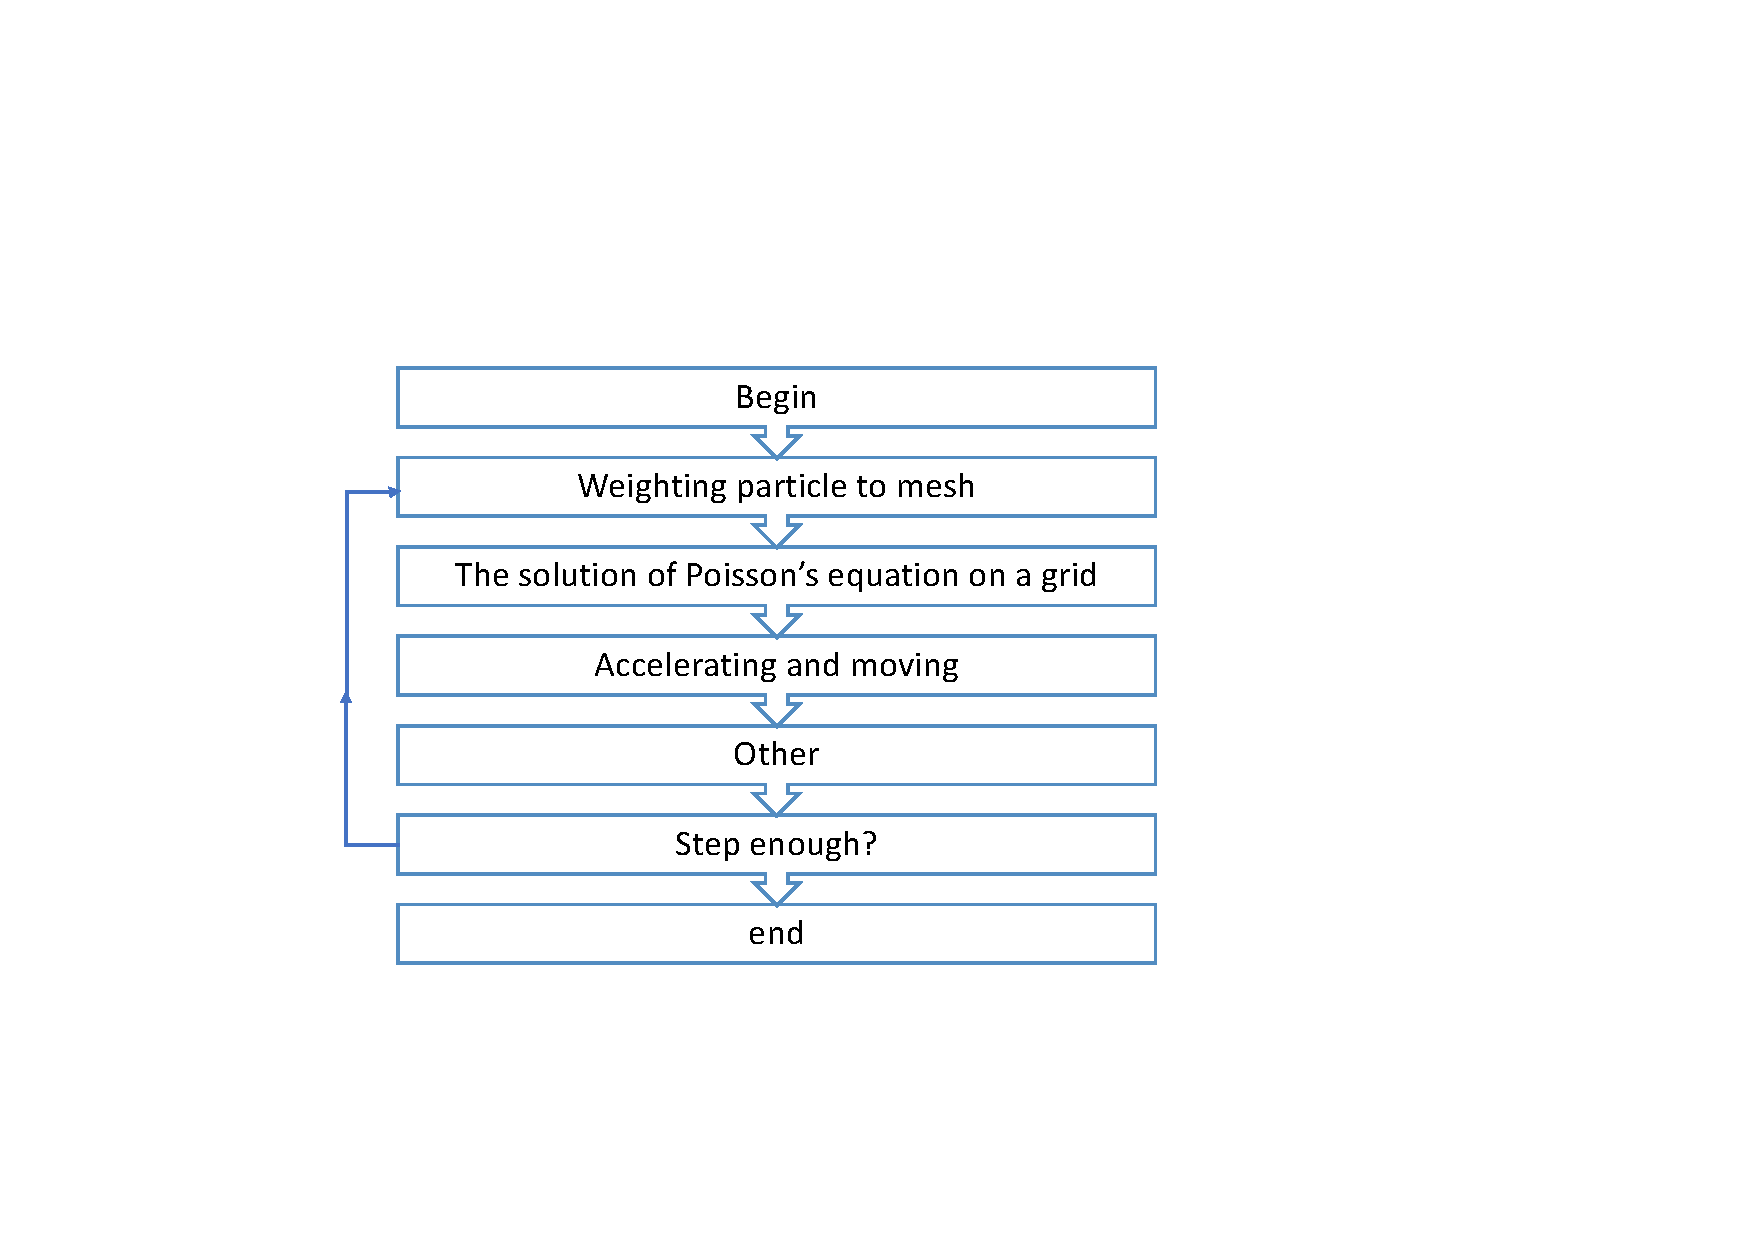
\includegraphics[width=0.7\textwidth]{Img/3_1_PIC2.pdf}
    \caption{PIC算法分段流程示意图}
    \label{fig:PICflow2}
\end{figure}

根据粒子的位置和范围确定所用的空间网格大小之后,模拟程序中的一步可以表示为:
\begin{enumerate}
  \item 将网格内的所有粒子的电荷根据粒子的位置权重到网格格点上,即从粒子分布得到获得空间点上的密度分布。
  \item 根据网格点上的电荷密度分布,求解网格点上的泊松方程,得到网格点上的电势分布。
  \item 根据电势分布,差分得到网格点上的电场分布。
  \item 根据粒子位置和网格上的电场分布,反向权重得到静止坐标系下粒子所受到的电场,再通过洛伦兹变换得到实验室坐标系下粒子所处位置的电磁场。
  \item 通过牛顿方程,推动粒子,更新粒子位置和动量。
\end{enumerate}

下面,我们分别就权重插值、空间电荷效应求解、粒子推动三个主要方面进行详细讨论。

\subsection{权重插值}
PIC算法的第一步是将粒子电荷权重插值到网格上。
粒子权重插值主要有以下几个方面进行考虑:

\begin{enumerate}
  \item 如何将粒子电荷密度(3D)或者电流密度(2D)权重到空间网格上。
  \item 求解泊松方程后,如何将网格上的电场权重插值回粒子上。
  \item 如何确定网格点的数目和相对于粒子分布的位置及范围。
\end{enumerate}

对于前两个问题,我们一般采用一个插值算法的正反两个过程来处理从粒子到网格和从网格到粒子的插值,从而避免算法上带来的非物理效应。如果采用不同的插值方法,可能会出现粒子自推动的错误。

以一维问题为例,将粒子电荷权重到空间网格上的过程,可以理解为粒子坐标$x_i$到网格点上的电荷密度$\rho_p$的一个映射,其中$p$为网格点的坐标。一些常见的权重方法如图\eqref{fig:PIC_weighting}所示,有最近网格点法(Nearest Grid Point, NGP)、网格差分法({Cloud In Cell, CIC)、以及三角云分配法(Triangular Shaped Cloud, TSC)。图中,粒子处于$x$位置,而$p-1$,$p$,$p+1$分别代表不同的网格格点,不同颜色的面积大小代表分配给相应格点的电荷权重,按照不同的形状分配可以得到不同的结果。
NGP方法为零阶插值,只将电荷分配到离粒子位置最近的网格点上,有较大误差;
CIC方法为一阶插值,根据粒子位置和格点位置的关系,如图\eqref{fig:PIC_CIC}所示,将粒子按不同比例分配到临近的两个网格点上;
TSC方法为二阶插值,如图\eqref{fig:PIC_TSC}所示,分配函数为三角形,将粒子按不同比例分配到临近的三个网格点上;
\begin{figure}[!htbp]
  \centering
  \begin{subfigure}[b]{0.8\textwidth}
    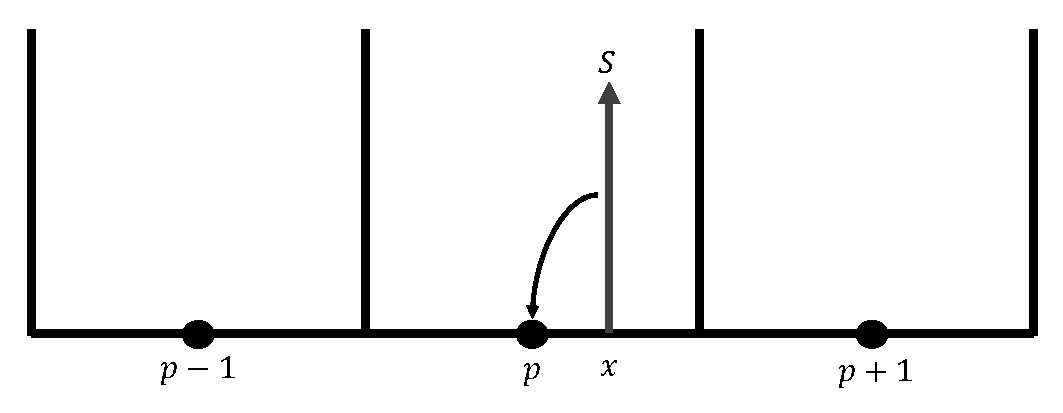
\includegraphics[width=\textwidth]{PIC_NGP}
    \caption{NGP}
    \label{fig:PIC_NGP}
  \end{subfigure}%
  ~%add desired spacing
  \begin{subfigure}[b]{0.8\textwidth}
    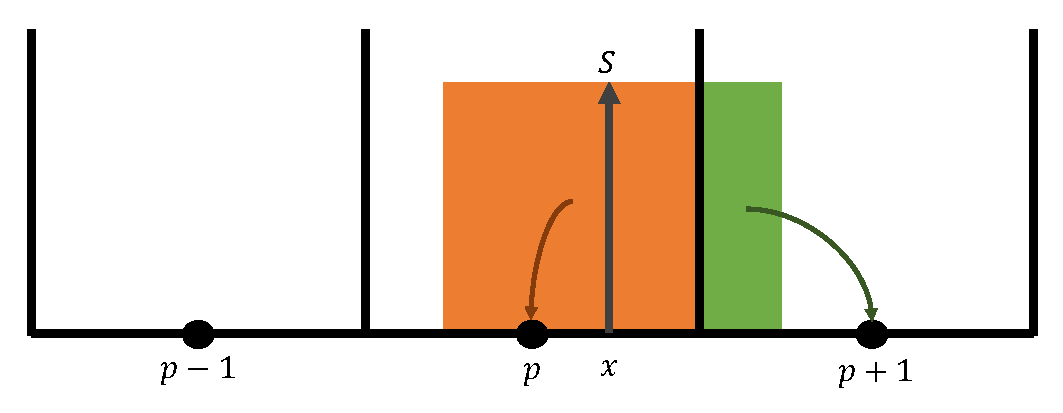
\includegraphics[width=\textwidth]{PIC_CIC}
    \caption{CIC}
    \label{fig:PIC_CIC}
  \end{subfigure}
  \begin{subfigure}[b]{0.8\textwidth}
    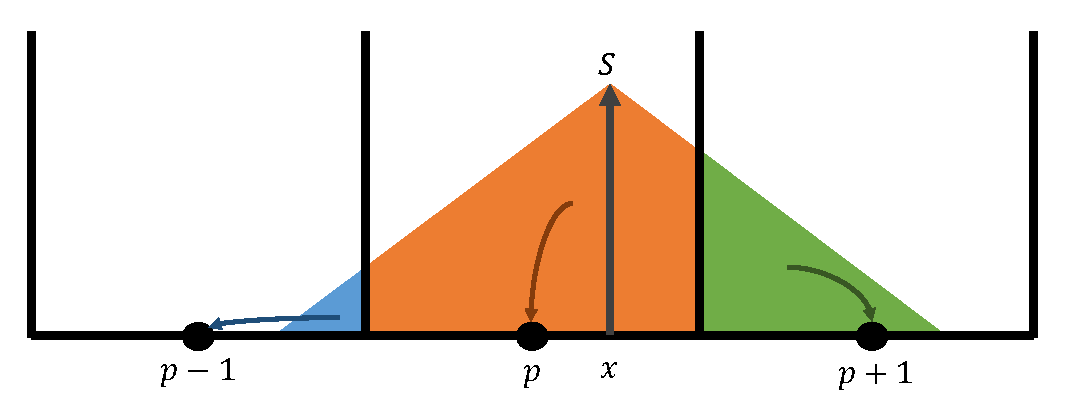
\includegraphics[width=\textwidth]{PIC_TSC}
    \caption{TSC}
    \label{fig:PIC_TSC}
  \end{subfigure}%
  \caption{权重插值中的分配方式示意图}
  \label{fig:PIC_weighting}
\end{figure}

在数学上,这个权重过程可以表示为:
\begin{equation}\label{eq:weight}
  \rho_p=\sum_{i}^{N_p} q_i W(x_i-x_p),
\end{equation}
其中,$q_i$为粒子所带电荷量,$W(x)$为形状因子。如图\eqref{fig:PIC_weighting2}所示,根据插值的阶数不同,$W(x)$有很多形式。下式给出了零阶,一阶,和二阶的形状因子:
\begin{equation}\label{eq:NGP}
  W_0(x)=\left\{
  \begin{aligned}
  &1, &\left| x \right| \leqslant \frac{\Delta x}{2}, \\
  &0, &\left| x \right| >         \frac{\Delta x}{2},
  \end{aligned}
  \right.
\end{equation}
\begin{equation}\label{eq:CIC}
  W_1(x)=\left\{
  \begin{aligned}
  &1-\frac{\left| x \right|}{\Delta x}, &\left| x \right| \leqslant \Delta x ,\\
  &0                                  , &\left| x \right| >         \Delta x ,
  \end{aligned}
  \right.
\end{equation}
\begin{equation}\label{eq:TSC}
  W_2(x)=\left\{
  \begin{aligned}
  &\frac{1}{ \Delta x} \left[\frac{3}{4}-(\frac{\left| x \right|}{\Delta x})^2 \right], &\left| x \right| \leqslant \frac{\Delta x}{2} ,\qquad \quad \\
  &\frac{1}{2\Delta x} \left[\frac{3}{2}- \frac{\left| x \right|}{\Delta x}    \right], &\frac{\Delta x}{2} < \left| x \right| \leqslant \frac{3\Delta x}{2}, \\
  &0,                                                                                   &\left| x \right| > \frac{3\Delta x}{2}\text{。}\qquad \ \
  \end{aligned}
  \right.
\end{equation}


\begin{figure}[!htbp]
  \centering
  \begin{subfigure}[b]{0.8\textwidth}
    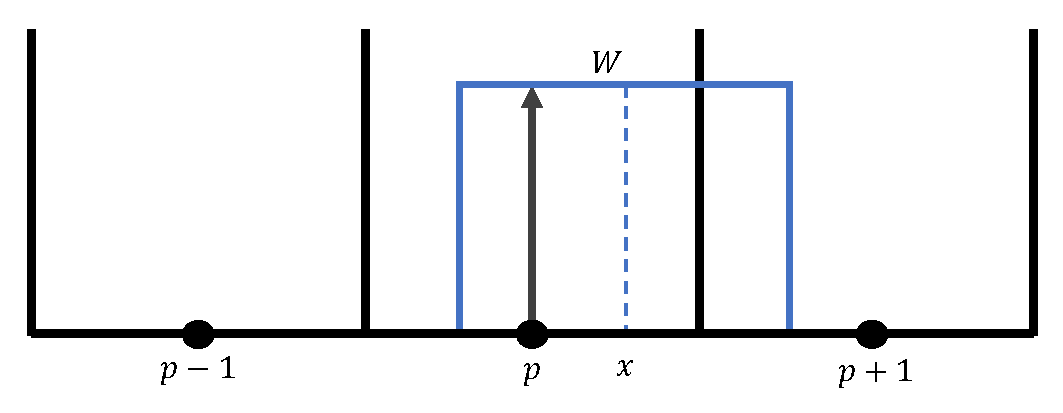
\includegraphics[width=\textwidth]{PIC_NGP2}
    \caption{NGP}
    \label{fig:PIC_NGP2}
  \end{subfigure}%
  ~%add desired spacing
  \begin{subfigure}[b]{0.8\textwidth}
    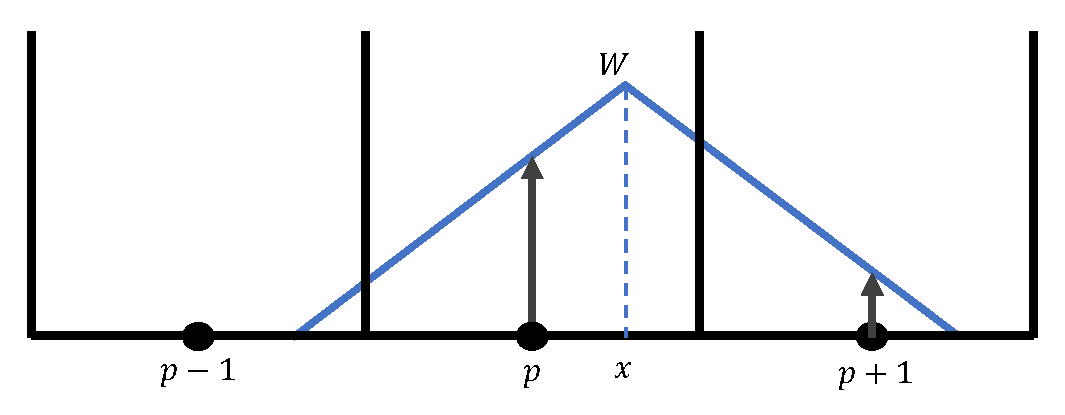
\includegraphics[width=\textwidth]{PIC_CIC2}
    \caption{CIC}
    \label{fig:PIC_CIC2}
  \end{subfigure}
  \begin{subfigure}[b]{0.8\textwidth}
    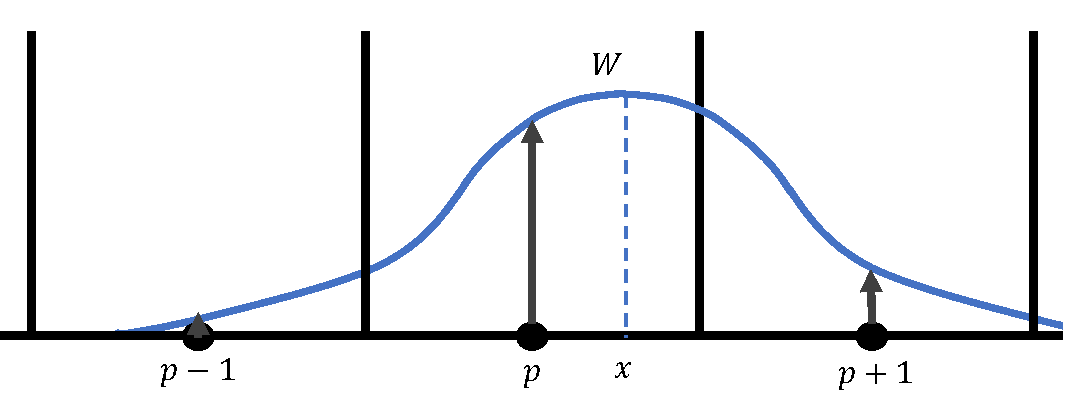
\includegraphics[width=\textwidth]{PIC_TSC2}
    \caption{TSC}
    \label{fig:PIC_TSC2}
  \end{subfigure}%
  \caption{权重插值中的形状因子曲线}
  \label{fig:PIC_weighting2}
\end{figure}

在数值模拟中,低阶的算法,比如NGP,会带来很大的粒子离散误差。为了避免数值误差,我们需要采取高阶精度的算法,但是高阶的算法会导致计算量的增大,不满足计算的要求。所以实际中往往采用CIC插值方法,兼顾精度和效率。在P-TOPO中,所有的插值形式都采用一阶的线性插值(CIC)。

对于实际的三维问题,处理方法也是类似,我们采用立方网格,使用体积权重法来计算网格上的电荷。

\subsection{使用FFT解泊松方程}
\label{section:PIC_FFT}
经过由粒子到空间网格的权重插值后,我们得到了分布在网格点上的电荷密度分布函数。接下来要做的就是求解网格点上的泊松方程,对于本程序而言,我们使用快速傅里叶变换(FFT)的方法来求解。以一维问题为例,泊松方程:
\begin{equation}\label{eq:Poisson}
\nabla^2 \phi = -\frac{\rho}{\epsilon _0},
\end{equation}
在网格上可以离散表示为:
\begin{equation}\label{eq:PoissonGrid}
\frac{\phi_{j-1}-2\phi_{j}+\phi_{j}}{\Delta _{x}^{2}}=-\frac{\rho _j}{\epsilon _0} \text{。}
\end{equation}
其中,$\phi_{j}$为第$j$个格点上的电势,$\rho_{j}$为第$j$个格点上的电荷量,$\Delta _{x}$为两个格点之间的距离。

将$\phi_{j}$和$\rho_{j}$进行展开,我们可以得到:
\begin{align}
\label{eq:FFT@phi}
\phi _j &= \frac{1}{N_x} \sum_{n=0}^{N_x}{\phi_n \exp{(-\frac{i2 \pi n j}{N_x} )}}, \\
\label{eq:FFT@rho}
\rho _j &= \frac{1}{N_x} \sum_{n=0}^{N_x}{\rho_n \exp{(-\frac{i2 \pi n j}{N_x} )}},
\end{align}
其中,$N_x$为一个方向上网格点的数目。
将式\eqref{eq:FFT@phi}和式\eqref{eq:FFT@rho}代回式\eqref{eq:PoissonGrid}可得:
\begin{equation}\label{eq:FFT@PIC2}
\begin{aligned}
\sum_{n=0}^{N_x}{\phi_n
\left(\exp{(-\frac{i2 \pi n (j-1)}{N_x} )}  -2\exp{(-\frac{i2 \pi n j}{N_x} )}  +  \exp{(-\frac{i2 \pi n (j+1)}{N_x} )}\right)} \\
= \frac{\Delta _{x}^{2}}{\epsilon _0} \sum_{n=0}^{N_x}{\rho_n \exp{(-\frac{i2 \pi n j}{N_x} )}}, \qquad\qquad\qquad
\end{aligned}
\end{equation}
对于傅里叶空间的电势和电荷密度,我们可以得到$\phi_{n}$和$\rho_{n}$的关系:
\begin{equation}\label{eq:FFT@PIC3}
\phi_{n}\left(\exp{(\frac{i2 \pi n}{N_x} )}  +  \exp{(-\frac{i2 \pi n}{N_x})} - 2 \right)
 = \frac{\Delta _{x}^{2}}{\epsilon _0} {\rho_n} \text{。} \\
\end{equation}
化简得到
\begin{equation}\label{eq:FFT@PIC3_consice}
\phi_{n} = \frac{\rho_n}{\epsilon _0 K_n^2}, \\
\end{equation}
其中
\begin{equation}\label{eq:FFT@PIC4}
K_n = (\frac{2\pi n}{N_x \Delta _x}) \frac{\sin({\pi n}/{N_x})}{{\pi n}/{N_x}}\text{。} \\
\end{equation}

可以看出,通过傅里叶变换得到的傅里叶空间中的电荷密度$\rho_{n}$,进而可以得到傅里叶空间中的电势分布函数$\phi_{n}$。然后再经过傅里叶逆变换,我们就可以得到实空间中的电势分布$\phi_{j}$,最后经过差分我们就可以得到空间电场分布函数。这个过程如图\eqref{fig:PIC_FFT_Poisson}所示。
\begin{figure}[ht]
  \begin{equation*}
    \centering
    \rho_j \quad \xrightarrow{\text{FFT}} \quad
    \rho_n \quad \xrightarrow{\text{Multiply by } \frac{1}{K_n^2}} \quad
    \phi_n \quad \xrightarrow{\text{IFFT}} \quad
    \phi_j \quad \xrightarrow{\text{Finite Difference}} \quad
    E_{x,j}
  \end{equation*}
  \caption{使用FFT求解泊松方程流程图}
  \label{fig:PIC_FFT_Poisson}
\end{figure}
需要注意的是,这种$e$指数的展开方式决定了我们使用的是周期性边界条件。如果我们想要第一类边界条件,我们需要采用$\sin$函数变换,其变换过程与此类似。
在P-TOPO中,我们在横向采用第一类边界条件,而在纵向采用周期性边界条件。

\subsection{蛙跳法推动粒子}
蛙跳法是一种束流模拟程序中常用的推动粒子的方法\cite{birdsall2004plasma},其计算的数学形式如下:
\begin{equation}
  \label{eq:leapfrog}
  \mathbf{v}_{i+3/2} = \mathbf{v}_{i+1/2} + \frac{\mathbf{F}(\mathbf{x}_{i+1})}{m} {\Delta T}
  ~, \qquad
  \mathbf{r}_{i+1}   = \mathbf{r}_{i}     + \mathbf{v}_{i+1/2} {\Delta T} \text{。}
\end{equation}
蛙跳法利用1/2时间步长处的粒子速度来推动粒子位置。
下面我们从一致性、同时性、高准确性、高稳定性四个方面来对蛙跳算法进行详细讨论。

\subsubsection{一致性}
      一致性是指差分方程和微分方程的一致。任何数值算法都是使用有限大小的步长来模拟一个连续的过程。
      因此,我们我们应该在时间步长无限小的时候,使其效果与连续推动一致。

      考虑经典的牛顿方程:
      \begin{align}
        \label{eq:PIC_push1}
         \frac{\mathrm{d} \mathbf{x}}{\mathrm{d} t} &= \mathbf{v} \text{,} \\
        \label{eq:PIC_push2}
        m\frac{\mathrm{d} \mathbf{v}}{\mathrm{d} t} &= \mathbf{F} \text{。}
      \end{align}
      如果我们采用有限步长$\Delta T$ 来推动粒子位置,牛顿运动方程变为:
      \begin{align}
         \label{eq:PIC_push3}
         \frac{\mathbf{x}_{n+1}-\mathbf{x}_n}{\Delta T} &= \mathbf{v}_n \text{,} \\
         \label{eq:PIC_push4}
        m\frac{\mathbf{v}_{n+1}-\mathbf{v}_n}{\Delta T} &= \mathbf{F}_n \text{。}
      \end{align}
      当其步长$\Delta T$足够小时,其结果应该与微分方程\eqref{eq:PIC_push1} 和\eqref{eq:PIC_push2}相一致。
\subsubsection{同时性}
      同时性又叫做可逆性。微分方程\eqref{eq:PIC_push1}和\eqref{eq:PIC_push2}是可逆的。
      例如,一个粒子在给定的力场中沿时间正向积分运动,然后如果将其速度取反,并沿时间反向积分,粒子将会沿着原有的轨迹向回运动,并能回到起始点。

      这一点在差分近似中并不能得到保证,比如,差分方程\eqref{eq:PIC_push3}和\eqref{eq:PIC_push4}中,粒子在第$n+1$步处取反,粒子位置变化为
      \begin{equation}
         \label{eq:PIC_push5}
         \frac{\mathbf{x}_{n}-\mathbf{x}_{n+1}}{\Delta T} = -\mathbf{v}_{n+1},
      \end{equation}
      其速度为$\mathbf{v}_{n+1}$而不是$\mathbf{v}_{n}$,也就是说粒子并不能沿其轨迹回到初始位置。这是因为差分方程的左右的时间中心不相同。
      式\eqref{eq:PIC_push3}左侧,位置改变为$\mathbf{x}_{n+1}-\mathbf{x}_n$,
      是以$t_{n+1/2}$为时间中心的;而右侧$\mathbf{v}_n$是时间$t_{n}$ 时的速度。因此,我们需要将其改变为:
      \begin{align}
         \label{eq:PIC_push6}
         \frac{\mathbf{x}_{n+1}-\mathbf{x}_n}{\Delta T} &= \mathbf{v}_{n+1/2},  \\
         \label{eq:PIC_push7}
          m\frac{\mathbf{v}_{n+1/2}-\mathbf{v}_{n-1/2}}{\Delta T} &= \mathbf{F}_n \text{。}
      \end{align}
      这也就是蛙跳法,即位置的时间与速度的时间并不在统一时刻,而是采用相差半个步长,然后交替推动粒子的速度和位置,以满足同时性条件。
\subsubsection{准确性}

      准确性与一步计算中的数值解与解析解的误差有关。
      这个误差主要来源于两方面:
      第一,来自于计算机的精度,例如,计算程序中一般使用双精度浮点数,十进制下仅有十四或十五位有效数字;
      第二,来自于使用有限小的步长代表连续变量的截断误差。
      通常来讲,第一种来自计算机数值精度的误差非常小,如果算法是稳定的(关于稳定性的论述见下一条),这个误差是可以忽略的。第二种来自于有限小的步长的误差,可以由解析解与数值解的差值来表示,其差值通常与步长$\Delta T$的$n$ 次方$(\Delta T)^n$成正比,而不同算法之间的稳定性可由阶数$n$来表示。准确性越差,程序实际所需要的时间步长就越小,即程序的计算效率越差。

      由式\eqref{eq:PIC_push6}和\eqref{eq:PIC_push7} 可知,蛙跳法为解析解\eqref{eq:PIC_push1}和\eqref{eq:PIC_push2}的二阶近似。证明如下:由式\eqref{eq:PIC_push6} 和\eqref{eq:PIC_push7}可得:
      \begin{equation}
         \label{eq:leapfrog_accuracy}
         \frac{\mathbf{x}_{n+1}-2\mathbf{x}_{n}+\mathbf{x}_{n-1}}{(\Delta T)^2} = \frac{\mathbf{F}(\mathbf{x}_n)}{m} \text{。}
      \end{equation}
      如果$\mathbf{X}$为解析解:
      \begin{equation}
         \label{eq:leapfrog_accuracy2}
         \frac{\mathrm{d}^2 \mathbf{X}}{\mathrm{d} t^2} = \frac{\mathbf{F}}{m},
      \end{equation}
      那么有限小步长的误差可以由${\delta}^n$表示:
      \begin{equation}
         \label{eq:leapfrog_accuracy3}
         \frac{\mathbf{X}_{n+1}-2\mathbf{X}_{n}+\mathbf{X}_{n-1}}{(\Delta T)^2} = \frac{\mathbf{F}(\mathbf{X}_n)}{m} - {\delta}^n \text{。}
      \end{equation}
      将$\mathbf{X}_{n+1}$和$\mathbf{X}_{n-1}$泰勒在$\mathbf{X}_{n}=\mathbf{X}(t_n)$ 处展开,式\eqref{eq:leapfrog_accuracy3}可以写作:
      \begin{equation}
         \label{eq:leapfrog_accuracy4}
         \frac{\mathrm{d}^2 \mathbf{X}}{\mathrm{d} t^2} + \frac{(\Delta T)^2}{12} \frac{\mathrm{d}^4 \mathbf{X}}{\mathrm{d} t^4} + h.o.t. =  \frac{\mathbf{F}(\mathbf{X}_n)}{m} - {\delta}^n,
      \end{equation}
      其中 $h.o.t.$ 为高阶项(higher order term)。式\eqref{eq:leapfrog_accuracy3} 与式\eqref{eq:leapfrog_accuracy4}相减可得:
      \begin{equation}
         \label{eq:leapfrog_accuracy5}
         {\delta}^n = -\frac{(\Delta T)^2}{12} \frac{\mathrm{d}^4 \mathbf{X}}{\mathrm{d} t^4} + h.o.t. \text{,}
      \end{equation}
      即,蛙跳法为二阶准确度(${\delta}^n \propto (\Delta T)^2$),基本能够满足程序需求。
\subsubsection{稳定性}
稳定性与误差随时间的变化有关。即使算法每一步的误差非常小,最终误差也有可能由于累积效应导致变大。
在一个数值算法中,如果每一步的误差不会导致更大的累积误差,那么这个算法是稳定的。

下面,我们讨论蛙跳法的稳定性。根据式\eqref{eq:leapfrog_accuracy},如果我们给定$\mathbf{x}_0 = \mathbf{X}_0,\mathbf{x}_1 = \mathbf{X}_1$作为初始条件,不考虑误差的情况下,我们可以得到之后的一系列解$\mathbf{X}_2$, $\mathbf{X}_3$, $\mathbf{X}_4,...$,其中:
      \begin{align}
         \label{eq:leapfrog_stability1}
         \mathbf{X}_{2}-2\mathbf{X}_{1}+\mathbf{X}_{0} &= \frac{\mathbf{F}(\mathbf{X}_1)}{m} {(\Delta T)^2} \text{,} \\
         \label{eq:leapfrog_stability2}
         \mathbf{X}_{3}-2\mathbf{X}_{2}+\mathbf{X}_{1} &= \frac{\mathbf{F}(\mathbf{X}_2)}{m} {(\Delta T)^2} \text{。}
      \end{align}
然而,由于误差的存在,我们无法得到微分方程中的精确解$\mathbf{X}_2,\mathbf{X}_3,\mathbf{X}_4,...$,
而是会得到一系列含有误差的近似解$\mathbf{x}_2,\mathbf{x}_3,\mathbf{x}_4,...$:
      \begin{align}
         \label{eq:leapfrog_stability3}
         \mathbf{x}_{2}-2\mathbf{X}_{1}+\mathbf{X}_{0} &= \frac{\mathbf{F}(\mathbf{X}_1)}{m} {(\Delta T)^2} \text{,} \\
         \label{eq:leapfrog_stability4}
         \mathbf{x}_{3}-2\mathbf{x}_{2}+\mathbf{X}_{1} &= \frac{\mathbf{F}(\mathbf{X}_2)}{m} {(\Delta T)^2} \text{。}
      \end{align}
这样,在第二步处的误差为
      \begin{equation}
         \label{eq:leapfrog_stability5}
         {\epsilon}_2 = \mathbf{x}_2 -\mathbf{X}_2 \text{。}
      \end{equation}

在随后的每一步计算中,含有误差的近似结果都会被使用,我们需要知道的是${\epsilon}_2$是如何影响后续计算结果。由式\eqref{eq:leapfrog_stability3}和式\eqref{eq:leapfrog_stability4}可得:
      \begin{equation}
         \label{eq:leapfrog_stabilit6}
         (\mathbf{X}_{3}+{\epsilon}_3)-2(\mathbf{X}_{2}+{\epsilon}_2)+\mathbf{X}_{1} = \frac{\mathbf{F}(\mathbf{X}_2+{\epsilon}_2)}{m} {(\Delta T)^2} \text{。}
      \end{equation}
与式\eqref{eq:leapfrog_stability2}相比较,可得
      \begin{equation}
         \label{eq:leapfrog_stabilit7}
         {\epsilon}_3-2{\epsilon}_2 = \left(\mathbf{F}(\mathbf{X}_2+{\epsilon}_2)  -\mathbf{F}(\mathbf{X}_2) \right)\frac{{(\Delta T)^2}}{m} \text{。}
      \end{equation}
将上式右侧在$\mathbf{x}=\mathbf{X}_2$处进行泰勒展开:
      \begin{equation}
         \label{eq:leapfrog_stabilit8}
         {\epsilon}_3-2{\epsilon}_2 \approx {\epsilon}_2\left. \frac{\partial\mathbf{F}}{\partial\mathbf{x}}\right|_{\mathbf{x}=\mathbf{X}_2} \frac{{(\Delta T)^2}}{m} \text{。}
      \end{equation}
类似可得:
      \begin{equation}
         \label{eq:leapfrog_stabilit9}
         {\epsilon}_4-2{\epsilon}_3+{\epsilon}_2 = {\epsilon}_3\left. \frac{\partial\mathbf{F}}{\partial\mathbf{x}}\right|_{\mathbf{x}=\mathbf{X}_3} \frac{{(\Delta T)^2}}{m},
      \end{equation}
则第$n$步的误差为
      \begin{equation}
         \label{eq:leapfrog_stabilit10}
         {\epsilon}_{n+1}-2{\epsilon}_n+{\epsilon}_{n-1} = {\epsilon}_n \left. \frac{\partial\mathbf{F}}{\partial\mathbf{x}}\right|_{\mathbf{x}=\mathbf{X}_n} \frac{{(\Delta T)^2}}{m} \text{。}
      \end{equation}
上式并不能得到一个准确的误差递进关系,除非${\partial\mathbf{F}}/{\partial\mathbf{x}}$为常量。
由于我们的目标是判断算法是否稳定,而不是算法有多稳定,
所以我们考虑最坏的情况,使用~$-|{\partial\mathbf{F}}/{\partial\mathbf{x}}|_{max}$~代替~${\partial\mathbf{F}}/{\partial\mathbf{x}}$~,
其中的负号是因为我们假设所计算的问题是有限边界,而不是会延伸到无穷远。则误差随时间的变化方程为
      \begin{equation}
        \label{eq:leapfrog_stabilit11}
         {\epsilon}_{n+1}-2{\epsilon}_n+{\epsilon}_{n-1} = -\left| \frac{\partial\mathbf{F}}{\partial\mathbf{x}}\right|_{max} \frac{{(\Delta T)^2}}{m} {\epsilon}_n,
      \end{equation}
定义$\Omega^2 \equiv \frac{1}{m} \left| \frac{\partial\mathbf{F}}{\partial\mathbf{x}}\right|_{max} $,则
      \begin{equation}
         {\epsilon}_{n+1}-2{\epsilon}_n+{\epsilon}_{n-1} = -(\Omega \Delta T)^2 {\epsilon}_n,
         \label{eq:leapfrog_stabilit12}
      \end{equation}
其解的形式与振动方程形式类似,即${\epsilon}_n = {\lambda}_n = \exp(i\omega n \Delta T)$。两个特征解${\lambda}_+$和${\lambda}_-$为
      \begin{equation}
         \label{eq:leapfrog_stabilit13}
         {\lambda}_\pm = 1- \frac{(\Omega \Delta T)^2}{2}\pm \left[\frac{(\Omega \Delta T)^2}{2}\right]\left[1-\frac{4}{(\Omega \Delta T)^2}\right]^{1/2}\text{。}
      \end{equation}
对于算法而言,想要保证数值上稳定,其误差不能随着时间而变大,误差推动方程的特征解必须位于单位圆内,即$|\lambda| \leq 1$。
因此,我们必须使时间步长足够小,才能保证算法稳定,对于蛙跳法而言,我们必须使
      \begin{equation}
          \Delta T \leq \frac{2}{\Omega}\text{。}
      \end{equation}
%\subsection{效率}
%blabla...

总之,权重插值、空间电荷效应求解、反向权重插值、粒子推动构成了基于PIC算法的模拟程序的主要步骤,一个有效的PIC程序必须满足以上各个部分的要求。
%PIC算法是求解空间电荷效应非常快速有效的方法,在PIC算法中,粒子首先被根据位置权重到网格上,
%然后根据网格上的电荷密度求解泊松方程,得到网格上的电势,从而得到网格上的电场,再根据粒子位置反推出粒子所处位置的电场。
使用这种方法,计算复杂度由直接的粒子-粒子方法的 $N_p^2$ 降低到了$\alpha N_p + \beta N_{cells}\log{N_{cells}}$。其中 $N_p$ 是粒子数,而$N_{cells}$ 是网格点数目。

\section{Symplectic算法}          \label{section:symplectic_theory}
上一节中我们讨论了PIC算法,这种算法使用网格进行空间电势求解,不可避免的会带来网格热噪声,从而导致数值噪声引起的束流发射度增长。
目前加速器界常用的PIC算法并不能保证辛条件(symplectic),其计算会被引入非物理效应,并对最终的强流束流物理的分析和讨论带来一些干扰。
因此,在需要长程模拟(比如环形加速器)的物理分析中,我们需要一种保辛的算法。

一开始,Symplectic算法是为了保证哈密顿系统中的辛条件而被研究 \cite{symplectic_channel1990, symplectic_yoshida1990}。
最近,无网格Symplectic模型被引入到加速器研究中作为空间电荷求解器 \cite{symplectic_ji2017}。
这种模型并不利用网格,而是利用高阶分解来求解空间电荷效应。
相比PIC算法,这种方法能够显著的降低由于网格数值噪声带来的发射度增长。
然而,虽然能够保证辛条件,这种算法相比PIC算法也有缺陷,最显著的就是其计算量更大。
无网格算法的计算复杂度为 $\alpha N_p * N_{modes}$ ,其中$N_{modes}$为分解的阶数,在通常模拟中我们一般使用$16 \times 16 \times 16$ 阶,在这种配置下Symplectic算法花费的时间比典型的$64 \times 64 \times 64$个格点的PIC算法要高两到三个数量级。
所以我们必须提高这个算法的运行速度,以提高算法的实用性。
幸运的是,由于无网格算法很适合并行的特性,这种算法能够很好的被加速,并且有很好的可扩展性。
下面,我们简要介绍Symplectic算法的基本原理。

在束流动力学模拟中,当且仅当雅可比矩阵 $\mathbb{M}_i$ 满足以下条件时,传输矩阵 $\mathbf{M_i}$ 才是保辛的\cite{accelerator2004lee, accelerator2013chao}:
\begin{equation}
\mathbb{M}_{i}^{T} \mathbf{J} \mathbb{M}_{i}=\mathbf{J},
\end{equation}
其中,$\mathbf{J}$ 是如下 $6N\times6N$ 的矩阵:
\begin{equation}
\mathbf{J}=\left(
  \begin{array}{cc}
     \mathbf{0} & \mathbf{I} \\
    -\mathbf{I} & \mathbf{0} \\
  \end{array}
\right) \text{。}
\end{equation}

对于考虑空间电荷力的多粒子系统,哈密顿量可以写为:
\begin{equation}
H={{H}_{1}}+{{H}_{2}},
\end{equation}
其中
\begin{eqnarray}
% \nonumber to remove numbering (before each equation)
  {H}_{1} &=& \sum\limits_{i}{{p_{i}^{2}}/{2}\;}+\sum\limits_{i}{q\psi ({{r}_{i}})} \text{,} \\
  {H}_{2} &=& \frac{1}{2}\sum\limits_{i}{\sum\limits_{j}{q\varphi ({{r}_{i}},{{r}_{j}})}} \text{。}
\end{eqnarray}
这里,${{H}_{1}}$ 只包含外场信息,而 ${{H}_{2}}$ 只包括空间电荷效应。根据${{H}_{1}}$ 和 ${{H}_{2}}$ 得到的两个传输矩阵 ${\mathbf{M}_{1}}$和 ${{\mathbf{M}}_{2}}$,一个二阶传输矩阵$\mathbf{M}\left( \tau  \right)$可以被定义为
\begin{equation}
\mathbf{M}\left( \tau  \right)={\mathbf{M}_{1}}\left( \tau /2 \right){\mathbf{M}_{2}}\left( \tau  \right){\mathbf{M}_{1}}\left( \tau /2 \right) \text{。}
\end{equation}
如果$ {\mathbf{M}_{1}} $和$ {\mathbf{M}_{2}} $都是保辛的,那么$ \mathbf{M} $就是保辛的。在大多数加速器元件中,我们可以通过单粒子动力学获得相应的外场传输矩阵$ {\mathbf{M}_{1}} $,而内场传输矩阵$ {\mathbf{M} _ {2}} $可以写为:
\begin{eqnarray}
 {{r}_{i}}(\tau ) &=& {{r}_{i}}(0) \text{,} \\
 {{p}_{i}}(\tau ) &=& {{p}_{i}}(0)-\frac{\partial {{H}_{2}}(r)}{\partial {{r}_{i}}}\tau  \text{。}
\end{eqnarray}
其雅克比矩阵为:
\begin{equation}
{{\mathbb{M}}_{2}}=\left(
\begin{array}{cc}
   \mathbf{I} & \mathbf{0}  \\
   \mathbf{L} & \mathbf{I}  \\
\end{array} \right),
\end{equation}
其中
${{L}_{ij}}=\frac{\partial {{p}_{i}}(\tau )}{\partial {{r}_{j}}}=-\frac{{{\partial }^{2}}{{H}_{2}}(r)}{\partial {{r}_{i}}\partial {{r}_{j}}}\tau$
是一个对称矩阵,所以${{\mathbb{M}}_{2}}$满足保辛条件.

对于一个3D束团, ${{H}_{2}}$可以表示为:
\begin{equation}
{{H}_{2}}=\kappa {{\gamma }_{0}}\sum\limits_{i}{\sum\limits_{j}{\varphi ({{r}_{i}},{{r}_{j}})}},
\end{equation}
其中 $\kappa =q/(lm{{C}^{2}}\gamma _{0}^{2}{{\beta }_{0}})$,$l=C/\omega $。而在束流坐标系下的静电势可以由求解泊松方程得到:
\begin{equation}
\frac{{{\partial }^{2}}\phi }{\partial {{x}^{2}}}+\frac{{{\partial }^{2}}\phi }{\partial {{y}^{2}}}+\frac{{{\partial }^{2}}\phi }{\partial {{z}^{2}}}=-\frac{\rho }{{{\varepsilon }_{0}}},
\end{equation}
其边界条件为:
\begin{equation}
\left\{
\begin{array}{cc}
   \phi (x=0,y,z)=0 \text{,} & \phi (x=a,y,z)=0 \text{,} \\
   \phi (x,y=0,z)=0 \text{,} & \phi (x,y=b,z)=0 \text{,}  \\
   \phi (x,y,z=0)=0 \text{,} & \phi (x,y,z=c)=0 \text{。}  \\
\end{array}
\right.
\end{equation}
这里,$a$,$b$,$c$分别是X,Y,Z方向上的零电势边界长度。如果我们将$c$设的足够大,电势将在无穷远处为零。

泊松方程中的电势$\phi$和电荷密度$\rho$可以展开为:
\begin{eqnarray}
 \rho(x,y,z)&=&\sum\limits_{l=1}^{{{N}_{l}}}{\sum\limits_{m=1}^{{{N}_{m}}}{\sum\limits_{n=1}^{{{N}_{n}}}{{{\rho }^{lmn}}\sin ({{\alpha }_{l}}x)\sin ({{\beta }_{m}}y)\sin ({{\gamma }_{n}}z)}}}, \\
 \phi(x,y,z)&=&\sum\limits_{l=1}^{{{N}_{l}}}{\sum\limits_{m=1}^{{{N}_{m}}}{\sum\limits_{n=1}^{{{N}_{n}}}{{{\phi }^{lmn}}\sin ({{\alpha }_{l}}x)\sin ({{\beta }_{m}}y)\sin ({{\gamma }_{n}}z)}}},
\end{eqnarray}
其中 ${N}_{l}$,${N}_{m}$,${N}_{n}$分别为电势和电荷密度在X,Y,Z三个方向上展开的阶数,而 ${\rho }^{lmn}$和 ${\phi }^{lmn}$可以表达为:
\begin{eqnarray}
  {{\rho }^{lmn}}&=&\frac{8}{abc}\int\limits_{0}^{a}{\int\limits_{0}^{b}{\int\limits_{0}^{b}{\rho (x,y,z)\sin ({{\alpha }_{l}}x)\sin ({{\beta }_{m}}y)\sin ({{\gamma }_{n}}z)dxdydz}}}, \\
 {{\phi }^{lmn}}&=&\frac{8}{abc}\int\limits_{0}^{a}{\int\limits_{0}^{b}{\int\limits_{0}^{b}{\phi (x,y,z)\sin ({{\alpha }_{l}}x)\sin ({{\beta }_{m}}y)\sin ({{\gamma }_{n}}z)dxdydz}}},
\end{eqnarray}
其中
\begin{equation}
{{\alpha }_{l}}=\frac{l\pi }{a},{{\beta }_{m}}=\frac{m\pi }{b},{{\gamma }_{n}}=\frac{n\pi }{c}\text{。}
\end{equation}
将上面$\rho$和$\phi$的展开代入泊松方程,我们可以得到:
\begin{equation}
{{\phi }^{lmn}}=\frac{{{\rho }^{lmn}}}{{{\varepsilon }_{0}}(\alpha _{l}^{2}+\beta _{m}^{2}+\gamma _{n}^{2})}\text{。}
\end{equation}
据此,我们得到了粒子密度$ \rho $和电势$ \phi $之间的关系:
\begin{multline}
\phi (x,y,z)=\frac{1}{{{\varepsilon }_{0}}}\frac{8}{abc}\omega \times \\ \sum\limits_{j=1}^{{{N}_{j}}}{\sum\limits_{l=1}^{{{N}_{l}}}{\sum\limits_{m=1}^{{{N}_{m}}}{\sum\limits_{n=1}^{{{N}_{n}}}{\frac{\sin ({{\alpha }_{l}}{{x}_{j}})\sin ({{\beta }_{m}}{{y}_{j}})\sin ({{\gamma }_{n}}{{z}_{j}})\sin ({{\alpha }_{l}}x)\sin ({{\beta }_{m}}y)\sin ({{\gamma }_{n}}z)}{(\alpha _{l}^{2}+\beta _{m}^{2}+\gamma _{n}^{2})}}}}},
\end{multline}
其中 $\omega $ 是粒子的电荷。
于是哈密顿量 ${{H}_{2}}$可以表示为:
\begin{multline}
{{H}_{2}}=\frac{1}{{{\varepsilon }_{0}}}\frac{8}{abc}\omega \kappa {{\gamma}_{0}} \times \\
\sum\limits_{i=1}^{{{N}_{i}}}{\sum\limits_{j=1}^{{{N}_{j}}}{\sum\limits_{l=1}^{{{N}_{l}}}{\sum\limits_{m=1}^{{{N}_{m}}}{\sum\limits_{n=1}^{{{N}_{n}}}
{\frac{\sin ({{\alpha }_{l}}{{x}_{j}})\sin ({{\beta }_{m}}{{y}_{j}})\sin ({{\gamma }_{n}}{{z}_{j}})\sin ({{\alpha }_{l}}{{x}_{i}})\sin ({{\beta }_{m}}{{y}_{i}})\sin ({{\gamma }_{n}}{{z}_{i}})}{(\alpha _{l}^{2}+\beta _{m}^{2}+\gamma _{n}^{2})}}
}}}}\text{。}
\end{multline}

最终,我们得到了保辛的空间电荷传输矩阵 ${\mathbf{M}_{2}}$。 以X方向为例:
\begin{align}
&{{x}_{i}}(\tau )= {{x}_{i}}(0), \\
 \nonumber &{{p}_{xi}}(\tau )= {{p}_{xi}}(0)-\tau \frac{1}{{{\varepsilon }_{0}}}\frac{8}{abc}\omega \kappa {{\gamma }_{0}} \times \\
 &\sum\limits_{j=1}^{{{N}_{j}}}{\sum\limits_{l=1}^{{{N}_{l}}}{\sum\limits_{m=1}^{{{N}_{m}}}{\sum\limits_{n=1}^{{{N}_{n}}}{\frac{{{\alpha }_{l}}\sin ({{\alpha }_{l}}{{x}_{j}})\sin ({{\beta }_{m}}{{y}_{j}})\sin ({{\gamma }_{n}}{{z}_{j}})\cos ({{\alpha }_{l}}{{x}_{i}})\sin ({{\beta }_{m}}{{y}_{i}})\sin ({{\gamma }_{n}}{{z}_{i}})}{(\alpha _{l}^{2}+\beta _{m}^{2}+\gamma _{n}^{2})}}}}}\text{。}
 \label{eq:symplectic_map1}
\end{align}
在Y和Z方向对应的粒子推动方程的形式与之类似。

\section{小结}                    \label{section:Algorithm_conclusion}
本章介绍了几种描述和求解空间电荷效应的模型。
早期的束核模型使用稳定束核假设,并对空间电荷力进行了线性近似,是一个非自洽的模型。
只能在一定程度上定性解释束晕形成的机制,而无法定量的求解出实际加速器中的空间电荷效应的影响。

PIC算法是一个更加自洽的用来描述空间电荷效应的方法。
束流模拟程序广泛的采用PIC算法来求解空间电荷力,
在PIC算法中,粒子首先根据位置被权重到网格上,
然后在网格上的求解泊松方程,以得到网格上的电势,
再根据粒子位置反推出粒子所处位置的电场。
PIC有效地降低了计算量,成为了国际上主流的空间电荷效应算法。
束流模拟程序一般使用蛙跳法来推动粒子,其满足一致性、同时性、高准确性、高稳定性四个条件。

然而,由于PIC算法含有网格热噪声,会被引入一些非物理效应,我们引入了Symplectic模型。
这种模型利用对粒子的高阶分解来求解空间电荷效应。
相比 PIC 算法, Symplectic 模型计算量要大得多,但是能够显著的降低~PIC算法中由于网格热噪声带来的发射度增长。

由于Symplectic算法计算量巨大,PIC算法也有提高效率的需求,我们需要对模拟程序进行并行化处理。
在下一章中,我们将对程序整体架构和各种算法在不同的并行计算平台上的实现进行介绍。


